% !TEX program = pdflatex
\documentclass[11pt,a4paper]{article}

% --- Page margins and paragraphs ---
\usepackage[margin=1in]{geometry}
\usepackage{parskip}

% --- Basic math and typesetting ---
\usepackage{amsmath,amssymb,amsthm}
\usepackage{xcolor} %

% --- Theorem and definition environments ---
\theoremstyle{definition}
\newtheorem{definition}{Definition}
\newtheorem{example}{Example}

\theoremstyle{plain}
\newtheorem{theorem}{Theorem}
\newtheorem{proposition}{Proposition}
\newtheorem{lemma}{Lemma}

\usepackage{mathtools,booktabs,enumitem,graphicx,url}
\usepackage[hidelinks]{hyperref}
\setlength{\emergencystretch}{2em}
\setlist{topsep=4pt,itemsep=3pt,parsep=0pt}
\raggedbottom
\newcommand{\dd}{\,\mathrm{d}}
\newcommand{\C}{\mathbb{C}}

\begin{document}

% ==================================================
% Title and author information
% ==================================================
\begin{center}
    {\LARGE \textbf{Mathematics Method for Physics--Lecture 8}} \\[0.6em]
    {\large Complex Series: Preliminaries}
\end{center}

\vspace{-0.5em}
\noindent\rule{\textwidth}{0.5pt}
\vspace{0.3em}

\begin{center}
    Instructor: Zhaolong Han, SOCE, Shanghai Jiao Tong University;
\end{center}

\vspace{-0.6em}
\noindent Email: han.arkey@sjtu.edu.cn

\vspace{0.4em}
\noindent\rule{\textwidth}{0.5pt}

\vspace{0.8em}

Complex series extend real-series convergence to the complex plane.
Power series have an especially useful geometry: their interior
convergence region is a disk. We use that fact to justify algebraic
operations and differentiation, then derive Taylor's theorem from
Cauchy's integral formula.

\section{Complex Series}
For a sequence $z_n\in\C$, the series $\sum_{n=1}^{\infty}z_n$ converges
to $S$ if its partial sums
\begin{equation}\label{eq:01}
S_N\coloneqq \sum_{n=1}^{N}z_n
 \quad\hbox{satisfy}\quad \lim_{N\to\infty}S_N=S\in\C.
\end{equation}
Otherwise it diverges. A finite complex limit is required.

\subsection{The geometric series}
For $z\neq1$,
\begin{equation}\label{eq:02}
\sum_{k=0}^{N}z^k=\frac{1-z^{N+1}}{1-z}.
\end{equation}
When $|z|<1$, $z^{N+1}\to0$, giving
\begin{equation}\label{eq:03}
\boxed{\frac1{1-z}=\sum_{n=0}^{\infty}z^n,\qquad |z|<1.}
\end{equation}
For $|z|\geq1$, the terms do not tend to zero, so the series diverges.
More generally,
\begin{equation}\label{eq:04}
\frac1{a-b}=\frac1a\sum_{n=0}^{\infty}\left(\frac ba\right)^n,
 \qquad |b|<|a|.
\end{equation}

\subsection{Basic convergence facts}
\begin{enumerate}
 \item Convergence implies $z_n\to0$. The converse is false; for example,
       $\sum_{n=1}^{\infty}1/n$ diverges.
 \item If $z_n=\alpha_n+\mathrm{i}\beta_n$, then $\sum z_n$ converges if and only if
       both real series $\sum\alpha_n$ and $\sum\beta_n$ converge.
 \item If $\sum|z_n|<\infty$, then $\sum z_n$ converges absolutely.
       A convergent series that is not absolutely convergent is called
       conditionally convergent.
\end{enumerate}
The real-series convergence tests can thus be applied to $\sum |z_n|$.
The componentwise statement follows by taking real and imaginary parts
of the partial sums. Absolute convergence implies that both component
series are absolutely convergent, since $|\alpha_n|,|\beta_n|\leq|z_n|$.

\section{Power Series and the Radius of Convergence}
A power series centered at $z_0$ has the form
\begin{equation}\label{eq:05}
\sum_{n=0}^{\infty}c_n(z-z_0)^n.
\end{equation}
Initially take $z_0=0$. Abel's convergence result states:
\begin{itemize}
 \item convergence at $z_1\neq0$ implies absolute convergence for
       every $|z|<|z_1|$;
 \item divergence at $z_2$ implies divergence for every $|z|>|z_2|$.
\end{itemize}
For the first claim, convergence at $z_1$ makes $c_n z_1^n$ bounded,
say by $M$. If $|z|<|z_1|$, then
\begin{equation}\label{eq:06}
|c_nz^n|\leq M\left|\frac z{z_1}\right|^n,
\end{equation}
and comparison with a geometric series proves absolute convergence.
For the second claim, convergence at a point of larger modulus would,
by the first claim, force convergence at $z_2$, a contradiction.

There is a radius $R\in[0,\infty]$ such that the power series converges
absolutely for $|z-z_0|<R$ and diverges for $|z-z_0|>R$.
Points on $|z-z_0|=R$ must be checked separately. If $R=0$, only the
center is included; if $R=\infty$, the series converges everywhere.



\begin{figure}[htbp]
\centering
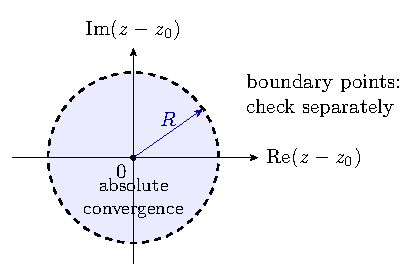
\includegraphics[width=.72\linewidth]{figs/fig08-01-radius-of-convergence.pdf}
\caption{Disk of absolute convergence; boundary points require separate tests.}
\label{fig:fig08-01-radius-of-convergence}
\end{figure}



The general radius formula is
\begin{equation}\label{eq:07}
\boxed{\frac1R=\limsup_{n\to\infty}|c_n|^{1/n}.}
\end{equation}
If either of the following limits exists, it may be used instead:
\begin{equation}\label{eq:08}
R=\frac1{\displaystyle\lim_{n\to\infty}|c_n|^{1/n}},
 \qquad
 R=\frac1{\displaystyle\lim_{n\to\infty}|c_{n+1}/c_n|}.
\end{equation}
The ratio expression assumes the ratios are eventually defined.
We use $1/0=\infty$ and $1/\infty=0$ for these formulas.

\section{Operations on Power Series}
Power series converge uniformly on every closed disk strictly inside their
disk of convergence. This is the condition that justifies the following
operations in the common interior disk. For example, choose
$0<r<\rho<R$. Convergence at $\rho$ makes $|c_n|\rho^n$ bounded,
so $|c_nz^n|\leq M(r/\rho)^n$ on $|z|\leq r$. The geometric
majorant gives uniform convergence on that closed disk.

For $A(z)=\sum a_nz^n$ and $B(z)=\sum b_nz^n$,
\begin{equation}\label{eq:09}
\begin{aligned}
 A(z)\pm B(z)&=\sum_{n=0}^{\infty}(a_n\pm b_n)z^n,\\
 A(z)B(z)&=\sum_{n=0}^{\infty}
     \left(\sum_{k=0}^{n}a_kb_{n-k}\right)z^n.
\end{aligned}
\end{equation}
The second formula is the Cauchy product.

If $b_0\neq0$, the quotient has a Taylor series in a sufficiently small
disk about $0$. Writing $A/B=\sum d_nz^n$ and comparing coefficients gives
\begin{equation}\label{eq:10}
d_0=\frac{a_0}{b_0},\qquad
 d_n=\frac{a_n-\sum_{k=1}^{n}b_kd_{n-k}}{b_0}\quad(n\geq1).
\end{equation}
This series represents $A/B$ on any centered disk on which $A,B$ are
holomorphic and $B$ has no zeros. Its convergence need not extend to the
whole common disk of $A$ and $B$: zeros of $B$ can obstruct it.

For $f(z)=\sum_{n=0}^{\infty}c_nz^n$ with radius $R$,
\begin{equation}\label{eq:11}
f'(z)=\sum_{n=1}^{\infty}n c_n z^{n-1},
 \qquad
 \int_0^z f(\zeta)\dd\zeta
    =\sum_{n=0}^{\infty}\frac{c_n}{n+1}z^{n+1},
 \qquad |z|<R.
\end{equation}
Both new power series have the same radius $R$. The integral can be taken
along any path from $0$ to $z$ lying inside the disk.

\section{Taylor's Theorem}
If $f$ is holomorphic in $|z-z_0|<R$, it has a unique expansion
\begin{equation}\label{eq:12}
\boxed{f(z)=\sum_{n=0}^{\infty}c_n(z-z_0)^n,\qquad
 c_n=\frac{f^{(n)}(z_0)}{n!},\quad |z-z_0|<R.}
\end{equation}
For any positively oriented circle $C_\rho:|\zeta-z_0|=\rho<R$,
\begin{equation}\label{eq:13}
c_n=\frac1{2\pi \mathrm{i}}\oint_{C_\rho}
              \frac{f(\zeta)}{(\zeta-z_0)^{n+1}}\dd\zeta.
\end{equation}
The case $z_0=0$ is called the Maclaurin expansion.

\subsection{Proof from Cauchy's integral formula}
Fix $z$ and choose $|z-z_0|<\rho<R$. On $C_\rho$,
\begin{equation}\label{eq:14}
\frac1{\zeta-z}
 =\frac1{\zeta-z_0}
    \frac1{1-(z-z_0)/(\zeta-z_0)}
 =\sum_{n=0}^{\infty}
       \frac{(z-z_0)^n}{(\zeta-z_0)^{n+1}}.
\end{equation}
The ratio has constant modulus $|z-z_0|/\rho<1$ on the integration
circle, so this geometric series is uniformly convergent there.
Cauchy's formula and termwise integration yield
\begin{equation}\label{eq:15}
\begin{aligned}
 f(z)&=\frac1{2\pi \mathrm{i}}\oint_{C_\rho}
                         \frac{f(\zeta)}{\zeta-z}\dd\zeta\\
 &=\sum_{n=0}^{\infty}
    \left[\frac1{2\pi \mathrm{i}}\oint_{C_\rho}
       \frac{f(\zeta)}{(\zeta-z_0)^{n+1}}\dd\zeta\right](z-z_0)^n.
\end{aligned}
\end{equation}
The higher-order Cauchy formula identifies the bracket as
$f^{(n)}(z_0)/n!$. Termwise differentiation at $z_0$ also shows that
these coefficients are unique.

The same argument gives an explicit remainder estimate. Let
$M_\rho=\max_{|\zeta-z_0|=\rho}|f(\zeta)|$. The finite geometric
identity in Cauchy's formula yields
\begin{equation}\label{eq:16}
\left|f(z)-\sum_{n=0}^{N}c_n(z-z_0)^n\right|
 \leq\frac{M_\rho\rho}{\rho-|z-z_0|}
       \left(\frac{|z-z_0|}{\rho}\right)^{N+1}.
\end{equation}
The right-hand side tends to zero because $|z-z_0|<\rho$.

Conversely, a convergent power series is holomorphic in its disk of
convergence. Thus a function is holomorphic on a domain if and only if
it has a convergent power-series representation in a neighborhood of
each point of that domain. A single series about one point need not
represent the function throughout an arbitrary domain.

\subsection{Standard expansions}
\begin{equation}\label{eq:17}
\begin{aligned}
 e^z&=\sum_{n=0}^{\infty}\frac{z^n}{n!},
 &\sin z&=\sum_{n=0}^{\infty}\frac{(-1)^nz^{2n+1}}{(2n+1)!},\\
 \cos z&=\sum_{n=0}^{\infty}\frac{(-1)^nz^{2n}}{(2n)!}.
\end{aligned}
\end{equation}
These three series converge for every $z\in\C$. For $|z|<1$,
\begin{equation}\label{eq:18}
\begin{aligned}
 \frac1{1-z}&=\sum_{n=0}^{\infty}z^n,\\
 \frac1{(1-z)^2}&=\sum_{n=0}^{\infty}(n+1)z^n,\\
 -\log(1-z)&=\sum_{n=1}^{\infty}\frac{z^n}{n}.
\end{aligned}
\end{equation}
Here $\log(1-z)$ is the holomorphic branch on $|z|<1$ with
$\log1=0$. The last two formulas follow by differentiating and
integrating the geometric series.

Worked Taylor expansions by direct differentiation and by reduction to
the geometric series are given in the exercise supplement.

\end{document}
